\documentclass[10pt]{article}

\usepackage[utf8]{inputenc}
\usepackage[T1]{fontenc}
\usepackage[polish]{babel}
\usepackage{listings}
\usepackage{xcolor}
\usepackage{amsmath, amssymb, amsthm}
\usepackage{graphicx}
\usepackage{geometry}
\usepackage{hyperref}
\usepackage{fancyhdr}
\usepackage{enumitem}
\usepackage{titlesec}
\usepackage[obeyspaces,spaces]{url}

\lstdefinestyle{base}{
  language=yaml,
  emptylines=1,
  breaklines=true,
  basicstyle=\ttfamily\color{black},
  moredelim=**[is][\color{red}]{@}{@},
}

\geometry{
    a4paper,
    left=25mm,
    right=25mm,
    top=25mm,
    bottom=25mm
}

\pagestyle{fancy}
\fancyhf{}
\fancyhead[L]{PW}
\fancyhead[R]{\thepage}
\fancyfoot[C]{}

\newtheorem{theorem}{Theorem}[section]
\newtheorem{lemma}[theorem]{Lemma}
\newtheorem{corollary}[theorem]{Corollary}
\newtheorem{definition}[theorem]{Definition}
\newtheorem{proposition}[theorem]{Proposition}
\newtheorem{remark}[theorem]{Remark}

\newcommand{\R}{\mathbb{R}}
\newcommand{\C}{\mathbb{C}}
\newcommand{\N}{\mathbb{N}}
\newcommand{\Z}{\mathbb{Z}}
\newcommand{\Q}{\mathbb{Q}}
\newcommand{\eps}{\varepsilon}
\newcommand{\norm}[1]{\left\lVert#1\right\rVert}
\newcommand{\abs}[1]{\left|#1\right|}

\titleformat{\section}{\normalfont\Large\bfseries}{\thesection}{1em}{}
\titleformat{\subsection}{\normalfont\large\bfseries}{\thesubsection}{1em}{}
\titleformat{\subsubsection}{\normalfont\normalsize\bfseries}{\thesubsubsection}{1em}{}

% Styl listingów.
\lstset{basicstyle=\footnotesize\ttfamily,breaklines=true}
\lstset{framextopmargin=50pt,frame=bottomline}

\title{Is RAG all you need?}
\author{Łukasz Ambroziak, Adam Kordeczka}

\begin{document}

\maketitle

\begin{abstract}
  Praca zaliczeniowa przedmiotu: \emph{Projektowanie rozwiązań Big Data} na kierunku: \emph{Big Data - przetwarzanie i analiza dużych zbiorów danych} organiozwanych przez Politechnikę Warszawską. Celem pracy było stworzenie skalowalnego, rozproszonego systemu umożliwiającego: (i) wykonywanie analiz ad-hoc z wykorzystaniem MongoDB, (ii) przetwarzenie danych wsadowych z wykorzystaniem Apache Spark, (iii) aplikowanie współczesnych metod przetwarzania języka naturalnego do efektywnego poszukiwania informacji, (iv) przygotowanie metod przeszukiwania dużego wolumenu danych tekstowych, które zasilą system Retrieval Augmented Generation (dalej: RAG). Część prezentacyjną uzupełnia interfejs graficzny umożliwiający komunikację z modelami uczenia maszynowego: DistilBERT oraz Phi-3. Repozytorium: \url{https://github.com/stasulam/pw-big-data-thesis-public}, live demo: \url{https://www.youtube.com/watch?v=FI0_qMbdIYs}.
\end{abstract}

\tableofcontents

\section{Wprowadzenie}

Motywacją dla przygotowania szytego na miarę systemu RAG było:

\begin{itemize}
  \item ocena możliwości stosowania systemów RAG jako alternatywy dla fine-tuningu dużych modeli językowych w rozwiązywaniu ściśle definiowanych zadań (często wymagających specjalistycznej wiedzy domenowej), np. udzielanie odpowiedzi w oparciu o aktualne akty prawne, udzielanie odpowiedzi z zakresu wąskich dziedzin wiedzy, itp.,
  \item przygotowanie modułowego, skalowalnego i elastycznego systemu, który będzie możliwy do stosowania w środowiskach o różnej dostępności zasobów obliczeniowych oraz pozwoli na niskokosztowe dostosowanie do konkretnego zadania - specjalizacja zamiast generalizacji,
  \item uniknięcie integracji z API dużych modeli językowych; celem było badanie możliwości stosowania mniejszych modeli językowych, które mogą być wdrażane w środowiskach on-premise bez dostępu do dużych zasobów obliczeniowych a jednocześnie realizować łącznie dwa cele: zwracać wysokiej jakości odpowiedzi oraz gwarantować prywatność przetwarzanych danych.
\end{itemize}

Stosowanie systemów RAG jako alternatywy dla dostrajania dużych modeli językowych jest obiecującym sposobem na korzystanie z nowoczesnych metod przetwarzania języka naturalnego w organizacjach pozbawionych dostępu do dużych zasobów obliczeniowych, finansowych lub braku kompetencji w uczeniu modeli tej klasy. Zauważmy, że Meta inwestuje 30 miliardów dolarów\footnote{\url{https://fusionchat.ai/news/metas-strategic-move-30-billion-investment-in-nvidia-gpus}} w zakup kart graficznych wykorzystywanych do budowy modeli uczenia maszynowego. Stanowi to 4.35\% polskiego Produktu Krajowego Brutto\footnote{\url{https://tradingeconomics.com/poland/gdp}} a więc więcej niż sumaryczne wydatki na obronność kraju na wschodniej flance NATO. Oczywistym wydaje się zatem, że uzyskanie przewagi konkurencyjnej i szybka adopcja technologii przetwarzania języka naturalnego będzie trudna do osiągnięcia na drodze bezpośredniej konkurencji z gigantami technologicznymi. W projekcie weryfikowaliśmy odmienny paradygmat dot. wykorzystania dużego modelu językowego. Zamiast tworzyć model wszechstronny przygotowaliśmy rozwiązanie wyspecjalizowane w realizacji konkretnego zadania z rezultatem lepszym niż wszechstronny model generatywny.

Zapewnienie modułowości motywowane jest przez dostosowywanie systemu do zastanego stosu technologicznego (w tym: kompetencji pracowników). W ramach projektu przygotowano rozwiązanie oparte o ugruntowane technologie (z pominięciem specjalizowanych frameworków), co może przyspieszyć ich adopcję w organizacjach. Jednocześnie w projekcie przedstawione zostaną propozycje w jaki sposób reguły eksperckie mogą wspierać systemy uczenia maszynowego we wskazywaniu obszarów, w których modele powinny poszukiwać odpowiedzi na zadane pytania.

Uniknięcie integracji z API dużych modeli językowych gwarantuje wysoką prywatność przetwarzanych danych. Współcześnie dane posiadane przez organizację stają się jej przewagą konkurencyjną. Udostępnienie tych danych, przez API, do wzbogacania dużych modeli językowych budowanych przez firmy zewnętrzne może finalnie ją zniwelować.

\section{Zbiór danych}

Zbiór danych wykorzystany w projekcie pochodzi z ArXiv\footnote{Od prawie 30 lat ArXiv służy zarówno społeczeństwu, jak i społecznościom naukowym, zapewniając otwarty dostęp do artykułów naukowych z różnych dziedzin, od rozległych obszarów fizyki po liczne subdyscypliny informatyki, a także wiele innych, w tym matematykę, statystykę, inżynierię elektryczną, biologię ilościową i ekonomię. Dostęp: \url{https://www.kaggle.com/Cornell-University/arxiv})}. Z uwagi na to, że oryginalny zbiór danych jest relatywnie duży (1.1 TB i rośnie) ograniczono się do wykorzystania pliku z metadanymi w formacie \texttt{json} (4.1 Gb). Plik ten zawiera wpis dla każdej pracy, zawierający:

\begin{itemize}
    \item \textbf{id}: identyfikator ArXiv (może być użyty do uzyskania dostępu do pracy, patrz poniżej),
    \item \textbf{submitter}: osoba, która zgłosiła pracę,
    \item \textbf{authors}: autorzy pracy,
    \item \textbf{title}: tytuł pracy,
    \item \textbf{comments}: dodatkowe informacje, takie jak liczba stron i rysunków,
    \item \textbf{journal-ref}: informacje o czasopiśmie, w którym praca została opublikowana,
    \item \textbf{doi}: \href{https://www.doi.org}{Cyfrowy Identyfikator Obiektu (DOI)},
    \item \textbf{abstract}: streszczenie pracy
    \item \textbf{categories}: kategorie / tagi w systemie ArXiv,
    \item \textbf{versions}: historia wersji;
\end{itemize}

Poniżej przedstawiono strukturę przykładowego dokumentu (ze zrandomizowanymi danymi):
\begin{lstlisting}
    {
        "root": {
            "id": "0704.0001",
            "submitter": "Jan Kowalski",
            "authors": "J. Kowalski",
            "title": "Hello, world!",
            "comments": "37 pages, 15 figures; published version",
            "journal-ref": "Phys.Rev.D76:013009,2007",
            "doi": "10.1103/PhysRevD.76.013009",
            "report-no": "ANL-HEP-PR-07-12",
            "categories": "hep-ph",
            "license": "MIT",
            "abstract": "Hello, world!",
            "versions": [0: {
              "version": "v1",
              "created": "Mon, 2 Apr 2007 19:18:42 GMT"
            }],
            "update_date": "2024-05-25",
            "authors_parsed": [0: [0: "J.", 1: "Kowalski"]]
        }
    }
\end{lstlisting}

\section{Architektura}

Rysunek \ref{fig:architecture} przedstawia architekturę systemu. System składa się z czterech głównych komponentów: (i) jeziora danych (ang. data lake), w którym dane przechowywane są w formie surowej, (ii) transformacji i ładowania danych z wykorzystaniem Apache Spark, (iii) przechowywania przetworzonych danych w nierelacyjnej bazie danych (MongoDB), (iv) części prezentacyjnej, w której użytkownik może przeszukiwać dane oraz korzystać z modeli uczenia maszynowego.

\begin{figure}[h]
    \centering
    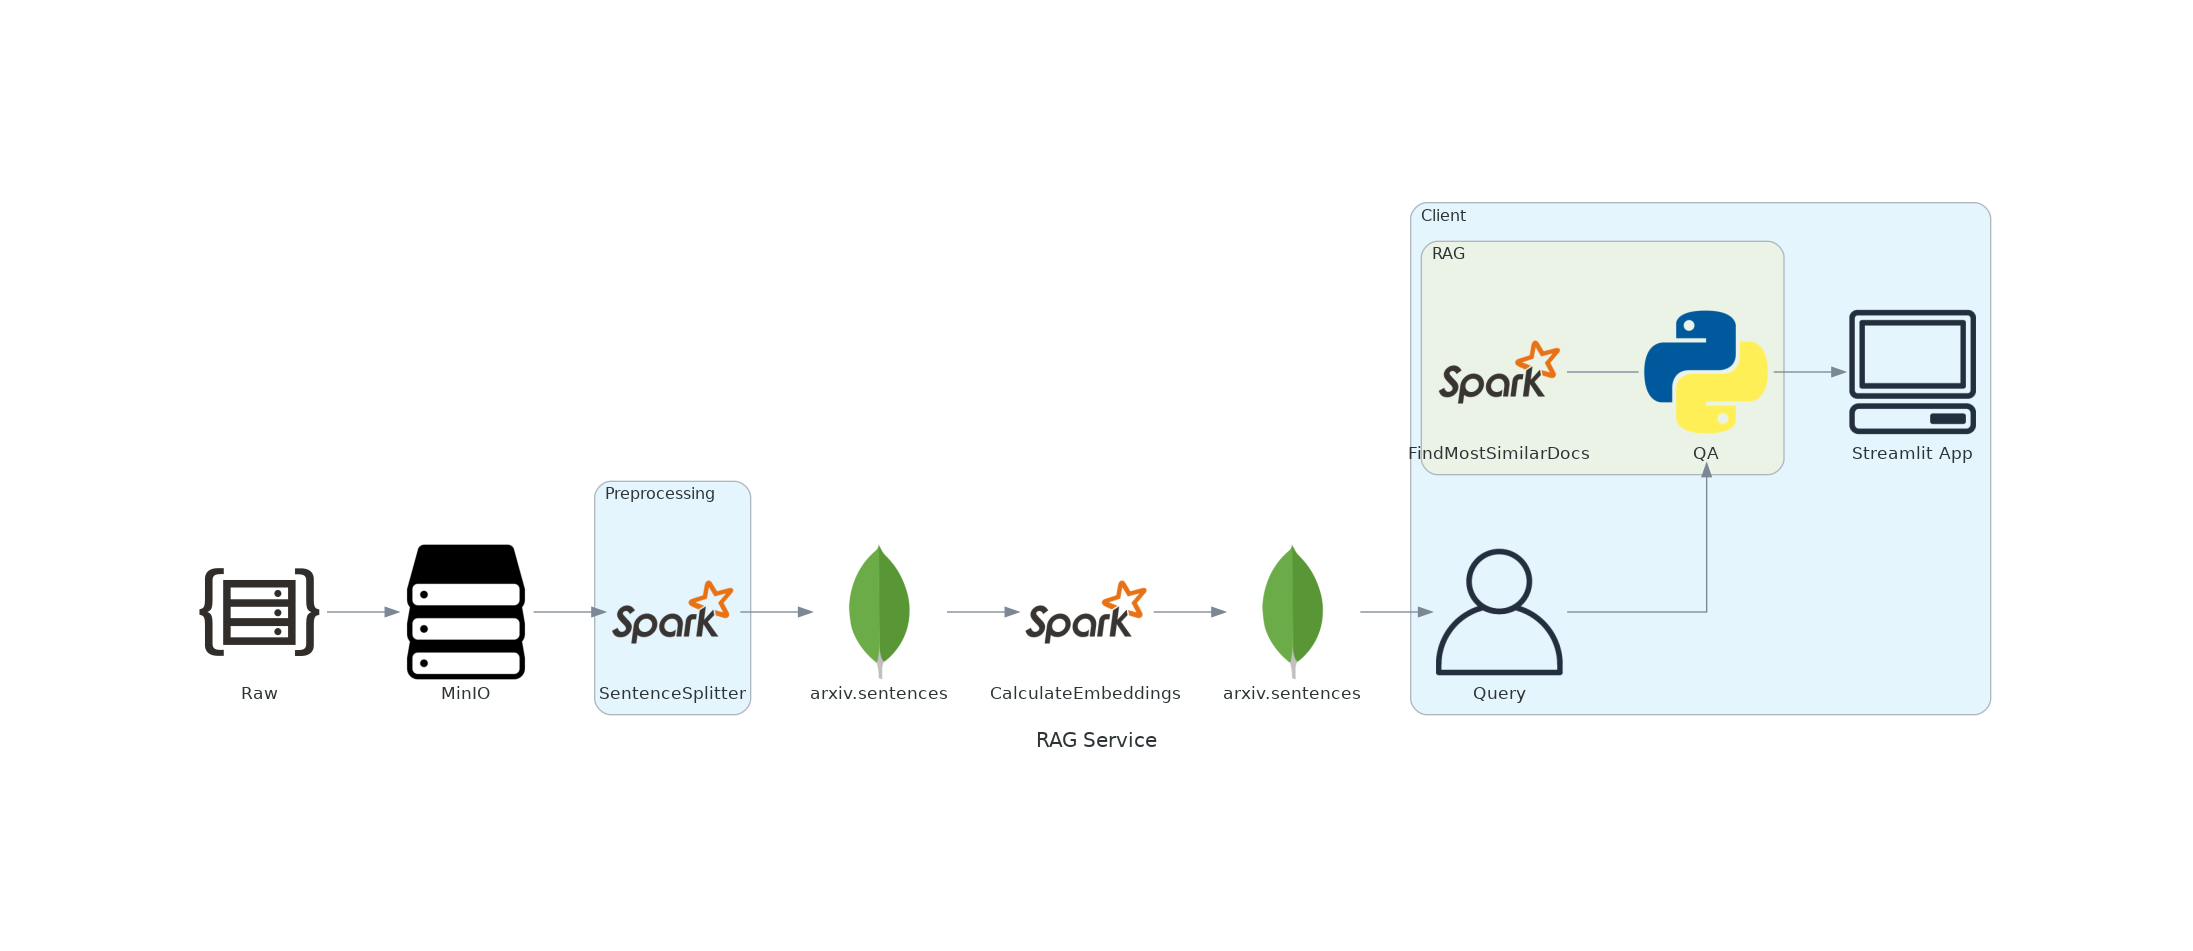
\includegraphics[width=1.0\textwidth]{images/architecture.png}
    \caption{Architektura systemu.}
    \label{fig:architecture}
\end{figure}

Infrastrukturę definiuje plik \texttt{docker-compose.yml}, który uruchamia kontenery z Apache Spark, MongoDB, MinIO, Jupyter. Plik załączono w \ref{s:docker-compose.yml}.

Interakcja z systemem odbywa się za pomocą pakietu Python o nazwie \texttt{rag}, który został zaimplementowany na potrzeby projektu. Pakiet posiada command-line interface implementujący następujące funkcjonalności:

\begin{lstlisting}
    # rag --help
    Usage: rag [OPTIONS] COMMAND [ARGS]...
    
    Options:
      --help  Show this message and exit.
    
    Commands:
      embeddings         Calculate embeddings.
      minio              Populate Minio with data.
      most-similar-docs  Get most similar documents.
      preprocessing      Preprocess data.
      qa                 Question & Answers.
\end{lstlisting}

\subsection{Jezioro danych}

W systemie jeziorem danych jest MinIO, który jest kompatybilny z Amazon S3. MinIO pozwala na przechowywanie danych w formie obiektów, które są dostępne za pomocą REST API. W projekcie dane przechowywane są w formie surowej w bucket \texttt{papers}. Każdy dokument zapisany jest w formacie JSON, gdzie nazwą pliku jest identyfikator ArXiv.

\subsubsection{Inicjalne zasilenie danych}

Rozpoczynamy od zasilenia systemu danymi. W tym celu korzystamy z polecenia \texttt{minio} w CLI pakietu \texttt{rag}:
\begin{lstlisting}
  Usage: rag minio [OPTIONS]

  Populate Minio with data.

  Args:
    path_to_raw_data (str): The path to the raw data.
    bucket (str): The name of the Minio bucket.
    processes (int): The number of processes to use for populating Minio.
    path_to_env (str): The path to the environment file.

  Returns: The result of the `main` function from 
    `rag.datasets.populate_minio`.

Options:
  --path-to-raw-data TEXT
  --bucket TEXT
  --processes INTEGER
  --path-to-env TEXT
  --help                   Show this message and exit.
\end{lstlisting}

Implementacja polecenia jest dostępna w repozytorium projektu w ścieżce \href{https://github.com/stasulam/pw-big-data-thesis-public/blob/main/src/rag/datasets/populate_minio.py}(\path{src/rag/datasets/populate_minio.py}).

Przykładowe użycie:
\begin{lstlisting}
  rag minio --path-to-raw-data data/raw/arxiv-metadata-oai-snapshot.json \
    --bucket papers \
    --processes 8 \
    --path-to-env .env
\end{lstlisting}

\subsubsection{Przechowywanie}

W MinIO przechowywane są surowe dane. Każdy dokument zapisany jest w formacie \texttt{json}. Dokumenty zapisywane są w folderach po 10 tys. dokumentów każdy. W efekcie uzyskujemy możliwość kontrolowania liczby wczytywanych dokumentów w zależności od dostępności zasobów obliczeniowych. W przypadku produkcyjnego wdrożenia systemu zakłada się przechowywanie nowopojawiających się dokumentów w folderach odpowiadających przedziałom czasowym, w którym dokumenty będą powstawały lub będą pobierane z zewnątrz. Umożliwi to łatwe zarządzanie danymi i harmonogramowanie przeliczeń z wykorzystaniem np. Apache Airflow.

\subsection{Transformacja i ładowanie danych}

Surowe dane z MinIO przetwarzane są z wykorzystaniem Apache Spark. W projekcie podjęto decyzję o przygotowywaniu reprezentacji wektorowych nie całej treści dokumentu (pole: \texttt{abstract}), ale pojedynczych zdań. Uzasadnienie: (i) reprezentacja wektorowa przygotowana na poziomie całego dokumentu może powodować utratę informacji niezbędną do powiązania danego dokumentu z treścią zapytania definiowanego przez użytkownika, (ii) użyteczna reprezentacja wektorowa pojedynczego zdania może być osiągnięta z wykorzystaniem mniejszego modelu, co pozwala na przetwarzanie danych również w warunkach mniejszej dostępności zasobów obliczeniowych.

Implementacja wstępnego przetwarzania danych dostępna jest w repozytorium projektu w ścieżce \href{https://github.com/stasulam/pw-big-data-thesis-public/blob/main/src/rag/processor/preprocessing.py}(\path{src/rag/processor/preprocessing.py}). Korzystamy z polecenia \texttt{preprocessing} w CLI pakietu \texttt{rag}:

\begin{lstlisting}
  Usage: rag preprocessing [OPTIONS]

  Preprocess data.

  This function performs data preprocessing using the specified data and
  environment paths.

  Args:
    path_to_data (str): The path to the data.
    path_to_env (str): The path to the environment.

  Returns: 
    The result of the preprocessing.

Options:
  --path-to-data TEXT
  --path-to-env TEXT
  --help               Show this message and exit.
\end{lstlisting}

Przykładowe użycie (małe zasoby obliczeniowe):
\begin{lstlisting}
  rag preprocessing --path-to-data s3a://papers/10k/*.json \
    --path-to-env .local-env
\end{lstlisting}

Przykładowe użycie (duże zasoby obliczeniowe):
\begin{lstlisting}
  rag preprocessing --path-to-data s3a://papers/*.json \
    --path-to-env .env
\end{lstlisting}

W efekcie przetworzone dane zostaną odłożone w MongoDB w bazie danych \texttt{arxiv} w kolekcji \texttt{sentences} w formie dokumentów o następującej strukturze:
\begin{lstlisting}
  {
    "_id": "0704.0001", # ArXiv ID
    "full_text": "Lorem ipsum dolor sit amet, consectetur adipiscing elit. ...", # Tresc abstraktu
    "sentences": [
      "Lorem ipsum dolor sit amet, consectetur adipiscing elit.",
      "..."
    ], # Zdania skladajace sie na tresc abstraktu
    "source": "s3a:/papers/10k", # Zrodlo danych
    "timestamp": "2024-06-04T19:38:02.486611", # Timestamp przetworzenia
  }
\end{lstlisting}

\subsection{Reprezentacje wektorowe}

Następnie, przygotowujemy reprezentacje wektorowe pojedynczych zdań. W tym celu korzystamy z modelu: \texttt{all-MiniLM-L6-v2}\footnote{\url{https://huggingface.co/sentence-transformers/all-MiniLM-L6-v2}}. W efekcie każde zdanie zostanie przekształcone do 384-elementowego wektora. Implementacja obliczania reprezentacji wektorowych dostępna jest w repozytorium projektu w ścieżce \href{https://github.com/stasulam/pw-big-data-thesis-public/blob/main/src/rag/processor/embeddings.py}(\path{src/rag/processor/embeddings.py}). Korzystamy z polecenia \texttt{embeddings} w CLI pakietu \texttt{rag}:

\begin{lstlisting}
  Usage: rag embeddings [OPTIONS]

  Calculate embeddings.

  This function calculates embeddings using the specified model.

  Args:
    path_to_env (str): The path to the environment.
    model (str): The name of the model to use.

  Returns: 
    The result of the `main` function from the `embeddings` module.

Options:
  --model TEXT
  --source TEXT
  --path-to-env TEXT
  --help              Show this message and exit.
\end{lstlisting}

Przykładowe użycie:
\begin{lstlisting}
  rag embeddings --model sentence-transformers/all-MiniLM-L6-v2 \
    --source s3a://papers/10k \
    --path-to-env .env
\end{lstlisting}

W efekcie dokumenty odłożone w MongoDB w bazie danych \texttt{arxiv} w kolekcji \texttt{sentences} zostaną uzupełnione o pole \texttt{embeddings}. Dokumenty będą miały następującą strukturę:

\begin{lstlisting}
  {
    "_id": "0704.0001", # ArXiv ID
    "full_text": "Lorem ipsum dolor sit amet, consectetur adipiscing elit. ...", # Tresc abstraktu
    "sentences": [
      "Lorem ipsum dolor sit amet, consectetur adipiscing elit.",
      "..."
    ], # Zdania skladajace sie na tresc abstraktu
    "source": "s3a:/papers/10k", # Zrodlo danych
    "timestamp": "2024-06-04T19:38:02.486611", # Timestamp przetworzenia,
    "embeddings": [
      Array(384),
      Array(384),
      ...,
    ] # Wektory reprezentujace zdania
  }
\end{lstlisting}

Korzystając z nierelacyjnej bazy danych, tj. MongoDB, w której dane przechowywane są w formie dokumentów, uzyskujemy możliwość elastycznego dodawania nowych pól do dokumentów. Gdy zainstnieje potrzeba o aktualizacji pól, np. o wynik działania modelu Named-Entity Recognition lub będziemy chcieli dodać nowe reprezentacje wektorowe, np. uzyskane z innego modelu, nie będziemy zmuszeni do zmian schematu bazy danych.

Naturalną ścieżką rozwoju projektu jest wersjonowanie modeli stosowanych do wyznaczania reprezentacji wektorowych, np. z wykorzystaniem MLFlow. W przypadku, gdybyśmy chcieli porównać jakość reprezentacji wektorowych uzyskanych z różnych modeli, moglibyśmy to zrobić w sposób zautomatyzowany.

\subsection{Poszukiwanie najbardziej podobnych dokumentów}

Na tym etapie dla zapytania zdefiniowanego przez użytkownika poszukiwane są dokumenty powiązane z zapytaniem, co de facto sprowadza się do stosowania algorytmu k-najbliższych sąsiadów z wykorzystaniem miary cosinusowej. Implementacja algorytmu dostępna jest w repozytorium projektu w ścieżce \href{https://github.com/stasulam/pw-big-data-thesis-public/blob/main/src/rag/processor/most_similar_docs.py}(\path{src/rag/processor/most_similar_docs.py}). Korzystamy z polecenia \texttt{most-similar-docs} w CLI pakietu \texttt{rag}:

\begin{lstlisting}
Usage: rag most-similar-docs [OPTIONS]

  Get most similar documents.

  Args:
    text (str): The input text.
    model (str): The name of the model to use.
    num_docs (int): The number of most similar documents to retrieve.
    query (str): The query to use for helping to retrieve the most 
      similar documents.
    path_to_env (str): The path to the environment.

  Returns:
    List[str]: A list of most similar documents.

Options:
  --text TEXT         [required]
  --model TEXT
  --num-docs INTEGER
  --query TEXT
  --path-to-env TEXT
  --help              Show this message and exit.
\end{lstlisting}

Dodatkowo: użytkownik może wesprzeć algorytm poszukiwania dokumentów poprzez zdefiniowanie zapytania, które ograniczy podzbiór dokumentów przez kwerendę stosowaną bezpośrednio w bazie danych MongoDB, tj. argument \texttt{query}.

\subsection{Część prezentacyjna}

\subsubsection{Aplikacja K-Y-D: \emph{Know-Your-Database}}

Część prezentacyjną systemu przygotowano wykorzystując bibliotekę \texttt{streamlit} w języku Python. Ułatwia ona tworzenie aplikacji webowych w szczególności związanych z uczeniem maszynowym i analizą danych.  

Całość składa się z trzech głównych widoków: \texttt{Basic info}, \texttt{QA} oraz \texttt{LLM}. Pierwsza z zakładek zawiera podstawowe informacje o bazie danych, na której działa RAG tj. jej liczebność oraz zrzut z treścią kilku przykładowych dokumentów. Rysunek \ref{fig:qa} przedstawia widok aplikacji KYD prezentujący funkcjonalność wykorzystania modelu ekstraktywnego w podejściu RAG.

\begin{figure}[h]
    \centering
    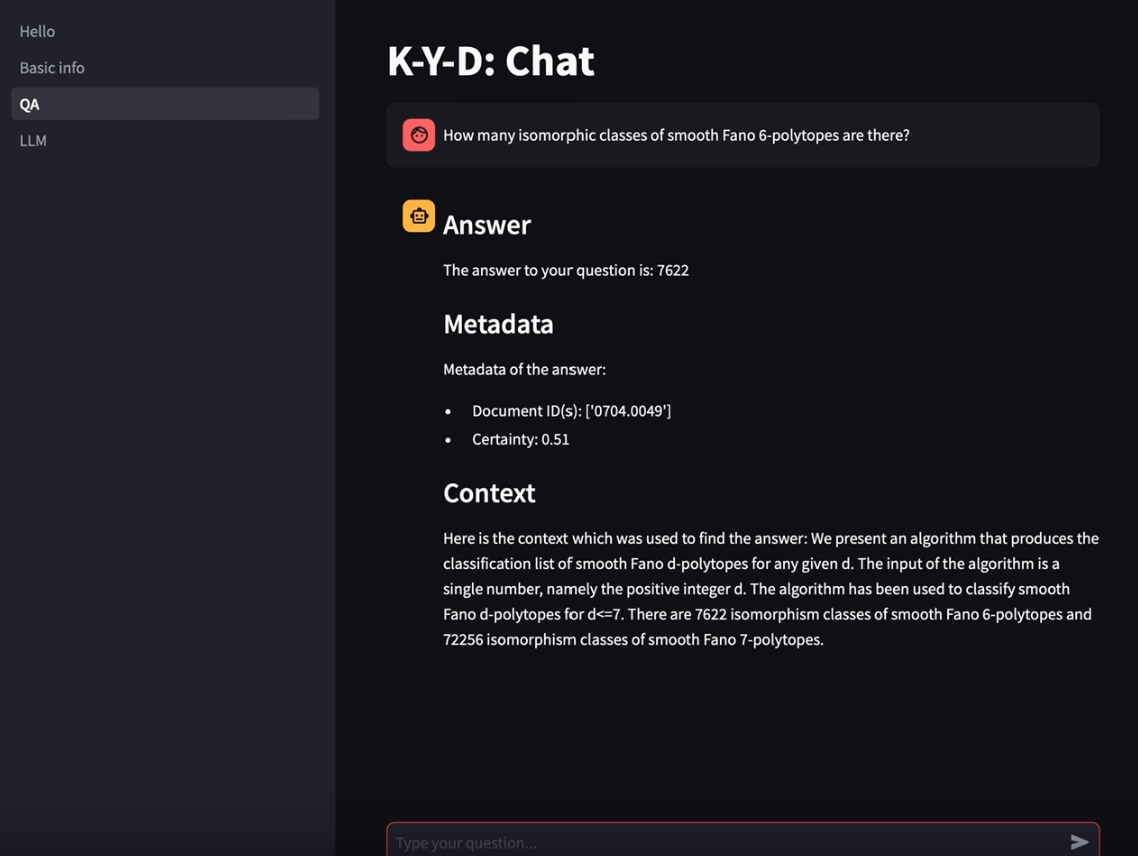
\includegraphics[width=1.0\textwidth]{images/QA-view.png}
    \caption{Widok zakładki QA.}
    \label{fig:qa}
\end{figure}

Użytkownik wchodzący w interakcje z aplikacją ma możliwość zadania pytania dotyczącego treści dokumentów, które zostały pobrane z bazy danych: \texttt{arxiv}, kolekcji: \texttt{senteces}. Zapytanie definiowane przez użytkownika jest zamieniane na reprezentację wektorową spójną z reprezentacjami wektorowymi przygotowanymi na wcześniejszych etapach. Następnie: poszukiwany jest 1-NN (ang. \emph{nearest neighbor}, najbliższy sąsiad) dla zapytania użytkownika. Treść całego dokumentu, którego zdanie jest najbardziej podobne do zapytania użytkownika, trafia do modelu: \texttt{distilbert\/distilbert-base-cased-distilled-squad}\footnote{https://huggingface.co/distilbert/distilbert-base-cased-distilled-squad}. Model zwraca odpowiedź na pytanie, identyfikator dokumentu na podstawie którego odpowiedź została udzielona oraz pewność z jaką udzielił odpowiedzi. Dodatkowo aplikacja została skonfigurowana w taki sposób, że jeśli pewność odpowiedzi nie przekracza progowego poziomu: 50\%, użytkownik przed uzyskaniem odpowiedzi na pytanie zostanie o tym ostrzeżony. Jest to jedna z metod rozwiązywania problemu halucynacji znanej z modeli generatywnych.

\begin{figure}[h]
    \centering
    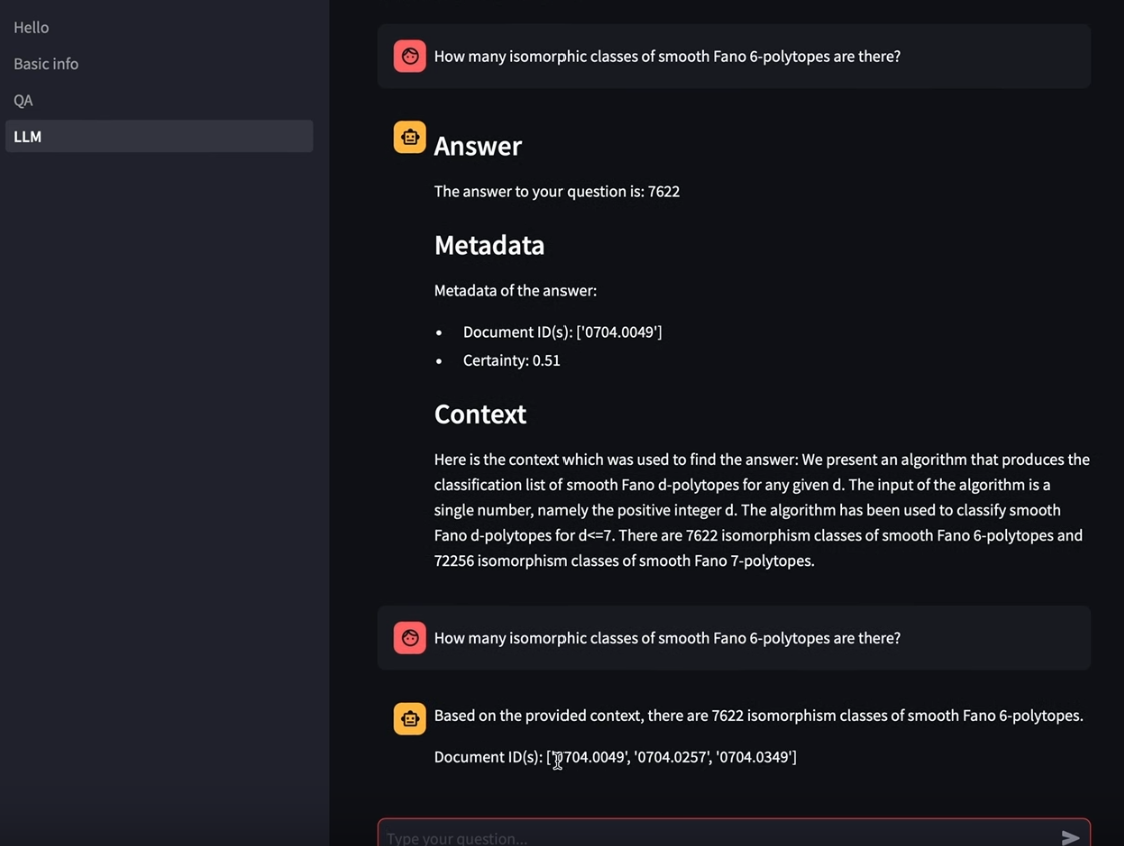
\includegraphics[width=1.0\textwidth]{images/LLM-view.png}
    \caption{Widok zakładki LLM.}
    \label{fig:llm}
\end{figure}

Rysunek \ref{fig:llm} przedstawia widok \emph{LLM}, którego funkcjonalność nie różni się co do zasady od poprzedniego. Zmianie ulega jednak model odpowiadający na zadane pytanie: w tym przypadku jest on abstraktywny tj. generuje sensowną i gramatycznie poprawną odpowiedź zawierającą odpowiedź na pytanie. 

Do działającego modelu LLM trafia następujący \textit{prompt}:

\begin{lstlisting}
"""
Context: ```
{context}
```
Given the context inside ``` solve the following taks: {task}.
If the context is not enough, try to solve the task with the
knowledge you have. But inform the user that the context is not
enough to solve the task.
"""
\end{lstlisting}

Dla przedstawionej na \ref{fig:llm} konfiguracji aplikacji w pole \textit{context} wklejane są trzy abstrakty, a w pole \textit{task} wklejane jest zadane przez użytkownika pytanie. Aplikacja zwraca odpowiedź wraz z ID trzech wykorzystanych w odpowiedzi abstraktach.

\subsubsection{Stosowane modele}

Do wyznaczenia reprezentacji wektorowych zapytań oraz zdań abstraktów wykorzystywany jest model \textbf{\textit{all-MiniLM-L6-v2}}, który na wyjściu zwraca 384-elementowy wektor. Jest to model zachowujący podstawową architekturę BERT, ale ze zmniejszonym rozmiarem i wymaganymi zasobami obliczeniowymi do jego sprawnego działania. 

W widoku \emph{QA} wykorzystano model \emph{\textbf{distilbert-base-cased-distilled-squad}} przystosowanego do zadań typu pytanie-odpowiedź. W widoku \emph{LLM} wykorzystano model \emph{\textbf{Phi-3-mini-4k-instruct-q4}} tj. LLM zbudowany przez \textit{Microsoft} adresujący problemy działania w środowisku o ograniczonej dostępności mocy obliczeniowej gwarantując jednocześnie odpowiednią jakość zwracanych rezultatów.


\section{Załączniki}

\subsection{docker-compose.yml}
\label{s:docker-compose.yml}

Niniejszy załącznik zawiera plik konfiguracyjny \texttt{docker-compose.yml} wykorzystywany przez silnik Docker Compose tj. narzędzie do zarządzania wielokontenerowymi aplikacjami. Uruchomienie aplikacji następuje po przejściu do głównego katalogu projektu i wywołaniu komendy \texttt{docker-compose up}. Powoduje to zbudowanie obrazów usług opisanych w pliku konfiguracyjnym, uruchomienie składowych serwisów i w konsekwencji całej aplikacji. Zatrzymanie działania usług następuje po wykonaniu komendy \texttt{docker-compose down}.

Każdy z wykorzystanych parametrów konfiguracyjnych został opisany w komentarzu odpowiadającym danej lini w pliku. 

\begin{lstlisting}

  version: '3.8' @#syntax version used by Docker Compose engine@

  services: @#'services' keyword defines list of services to be deployed@
  
    mongo: @#'mongo' service configuration chunk@
      image: mongo:latest @#docker image version pulled from dockerhub@
      container_name: mongodb @#working service name@
      ports: @#port mapping between docker machine and host@
        - "27017:27017" 
      volumes: @#storage volumes mounted to the machine filesystem@
        - ./data/mongo:/data/db
  
    spark: @#'spark' service configuration chunk@
      image: custom-spark:3.5.0
      build: @#building service using provided Dockerfile@
        context: .
        dockerfile: ./dockerfiles/spark
      container_name: spark
      environment: @#Environment variables passed to running container@
        - SPARK_MODE=master
        - SPARK_MASTER_HOST=spark
        - SPARK_MASTER_PORT=7077
        - SPARK_RPC_AUTHENTICATION_ENABLED=no
        - SPARK_RPC_ENCRYPTION_ENABLED=no
        - SPARK_LOCAL_STORAGE_ENCRYPTION_ENABLED=no
        - SPARK_SSL_ENABLED=no
        - XDG_CACHE_HOME=/opt/bitnami/spark/.cache
      ports:
        - "8080:8080"
        - "7077:7077"
  
    spark-worker: @#'spark-worker' service configuration chunk@
      image: custom-spark:3.5.0
      build:
        context: .
        dockerfile: ./dockerfiles/spark
      container_name: spark-worker
      environment:
        - SPARK_MODE=worker
        - SPARK_MASTER_URL=spark://spark:7077
        - SPARK_RPC_AUTHENTICATION_ENABLED=no
        - SPARK_RPC_ENCRYPTION_ENABLED=no
        - SPARK_LOCAL_STORAGE_ENCRYPTION_ENABLED=no
        - SPARK_SSL_ENABLED=no
        - XDG_CACHE_HOME=/opt/bitnami/spark/.cache
      depends_on: @#Specifies deployment dependency between services@
        - spark   @#i.e.'spark-worker' service starts after 'spark'@
        
  
    minio: @#'minio' service configuration chunk@
      image: minio/minio
      ports:
        - 9000:9000
        - 9001:9001
      environment:
        - MINIO_ROOT_USER=minio
        - MINIO_ROOT_PASSWORD=miniominio
      container_name: minio
      @#below determines 'command' executed inside container after start@
      command: server /data/minio --console-address ":9001"
      @#Below defines operation executed in order to assure that@
      @#the service is running properly. If 'healthcheck' fails the@
      @#deployment is aborted.@
      healthcheck:
        test:
          [
            "CMD",
            "curl",
            "-f",
            "http://localhost:9000/minio/health/live"
          ]
        interval: 30s
        timeout: 20s
        retries: 3
      volumes:
        - ./data/minio:/data/minio
  
    jupyter: @#'jupyter' service configuration chunk@
      image: jupyter:1.0.0
      container_name: jupyter
      build:
        context: .
        dockerfile: ./dockerfiles/jupyter
      ports:
        - "8888:8888"
        - "8501:8501" #streamlit app port
      command:
        [
          "jupyter",
          "lab",
          "--ip=0.0.0.0",
          "--port=8888",
          "--no-browser",
          "--allow-root",
          "--NotebookApp.token=''"
        ]
      volumes:
        - ./:/rag/
      depends_on:
        - mongo
        - spark
        - spark-worker
        - minio
  @#declaring volumes used to persist data generated by Docker container@
  volumes:
    mongo-data:
    minio-data:
  
\end{lstlisting}

\end{document}
